\subsection{Installazione di Grafana}
Per installare Grafana\glo, visitare la pagina \url{https://grafana.com/get}. Qui è possibile trovare il download per MacOS, Windows e sistemi operativi basati su Linux/Unix.
\subsubsection{Eseguire il servizio WEB Grafana} Per eseguire il servizio WEB Grafana\glo, aprire la cartella "bin" dell'installazione Grafana\glosp ed a seconda del sistema operativo eseguire:
\begin{itemize}
	\item \textbf{Windows}: doppio click sul file "grafana-server";
	\item \textbf{Linux e Mac}: eseguire in una shell il comando:
		\begin{verbatim}
			./grafana-server web
		\end{verbatim}
\end{itemize}
Collegarsi quindi con un browser all'indirizzo \url{http://localhost:3000/}. Le credenziali richieste al primo avvio sono username "admin" e password "admin".
\begin{figure}[H] 	
	\begin{center}
		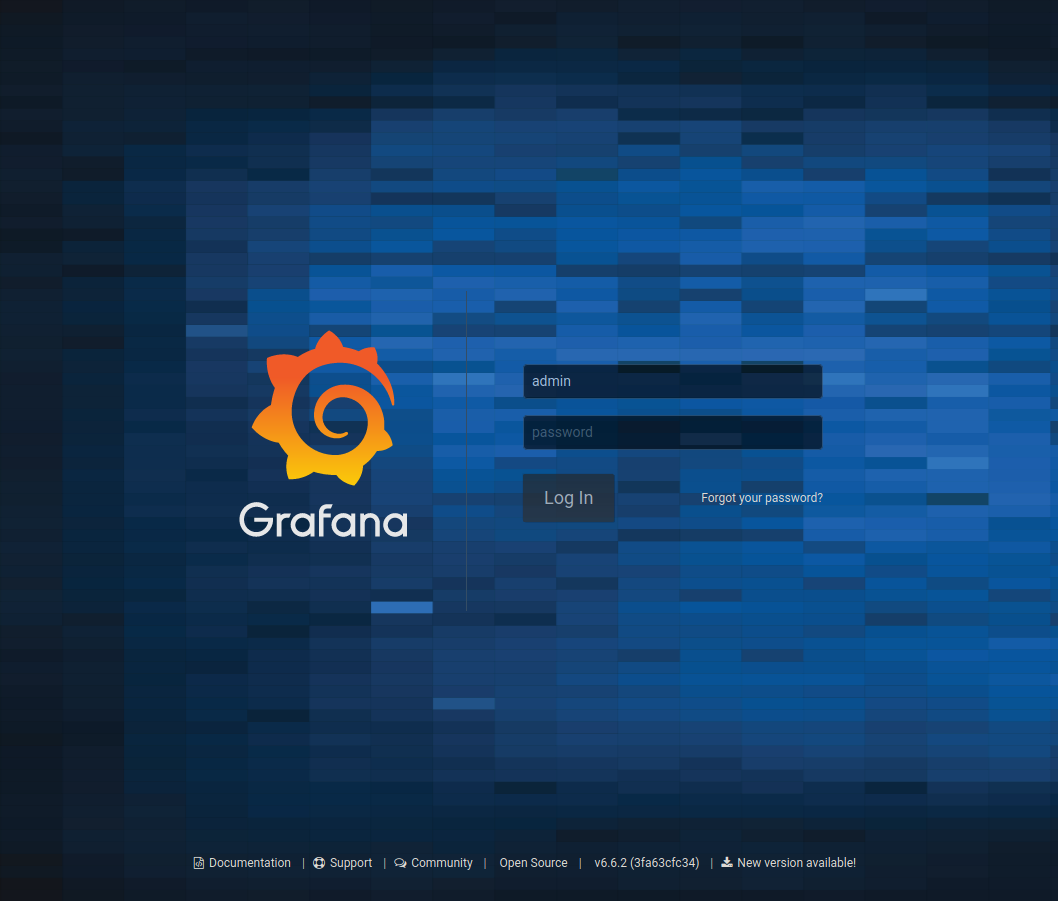
\includegraphics[width=10cm,height=\textheight,keepaspectratio]{img/grafana-login.png}
	\end{center}
	\caption{Pagina di login di Grafana}	
\end{figure}

%\subsection{Installazione plug-in Grafana}
%\subsubsection{Requisiti}
%\begin{itemize}
%	\item \textbf{Grafana\glo};
%	\item \textbf{Node.js}: runtime Javascript che permette di eseguire codice Javascript fuori da un browser. L'installazione di npm (Node Package Manager) non è richiesta dato che viene installato automaticamente durante l'installazione di Node.js;
%	\item \textbf{Git}: sistema di versionamento distribuito.
%\end{itemize}

\subsection{Installazione del plug-in}
\subsubsection{Clonare la repository da GitHub}%\mbox{}\\ [1mm]
Per clonare la repository dell'applicazione, aprire un terminale e usare il comando cd per spostarsi in una cartella a propria scelta ed eseguire il comando:
\begin{verbatim}
	git clone https://github.com/VRAM-Software/grafana_prediction.git
\end{verbatim}
Infine con il comando 
\begin{verbatim}
	cd ./grafana_prediction_plugin
\end{verbatim}
si accede alla cartella che contiene il codice sorgente del plug-in.

\subsubsection{Installare le dipendenze\glo}%\mbox{}\\ [1mm]
Per il corretto funzionamento dell'applicazione è necessario installare tutte le dipendenze\glosp elencate precedentemente. Per farlo eseguire il comando:
\begin{verbatim}
	npm install
\end{verbatim}

\subsubsection{Eseguire il plug-in}%\mbox{}\\ [1mm]
Per eseguire il plug-in è necessario copiare il contenuto del repository "grafana\_prediction\_plugin", ad eccezione delle cartelle "node\_modules" e "coverage", all'interno della cartella "data/plugins" dell'installazione Grafana\glo. Accedendo all'interfaccia web si potrà quindi abilitare il plug-in dall'apposita sezione plug-in delle impostazioni.
\\
\\
\begin{figure}[H] 	
	\begin{center}
		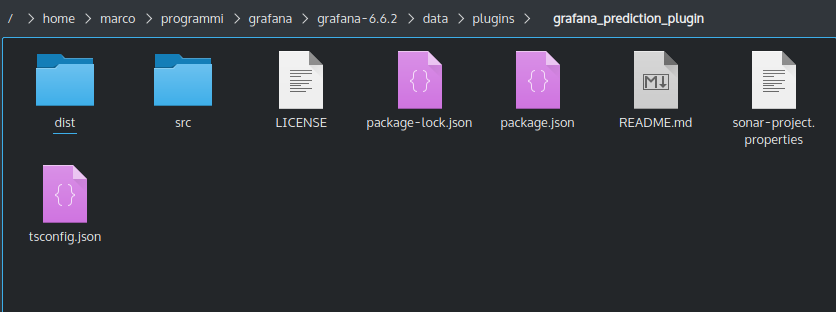
\includegraphics[width=\textwidth,height=\textheight,keepaspectratio]{img/plugin-directory.png}
	\end{center}
	\caption{Selezione plug-in nella directory}	
\end{figure}

\subsubsection{Impacchettare il plug-in}%\mbox{}\\ [1mm]
Per generare una release di produzione\glosp basta eseguire il comando:
\begin{verbatim}
	npm run build	
\end{verbatim}
e successivamente creare un archivio zip dell'intero repository escludendo le cartelle "node\_modules" e "coverage". Questo plug-in potrà poi essere distribuito e installato da altri utenti. 
